\documentclass[t,10pt]{beamer}
\usetheme[official=true,titlebgimage=toro,conference=\mbox{N. Vianello
  @ KTH 22 June 2011}]{rfx}
\usepackage[english]{babel}
\usepackage{listings,amsmath,multimedia}
\usepackage{tangocolors}
\usepackage{rfxcolor}
\usepackage{pgf}
\usepackage{tikz}
\usepackage[bibstyle=numeric-comp,citestyle=authoryear-comp,labelyear=true,maxnames=1]{biblatex}
\bibliography{biblio}
\renewcommand*{\bibfont}{\footnotesize}
\mode<presentation>
\graphicspath{{pdf_box/}}
\renewcommand\Re{\operatorname{Re}}
\renewcommand\Im{\operatorname{Im}}

% for adding foot note with reference
\makeatletter
% add a macro that saves its argument
\newcommand{\footlineextra}[1]{\gdef\insertfootlineextra{#1}}
\newbox\footlineextrabox

% add a beamer template that sets the saved argument in a box.
% The * means that the beamer font and color "footline extra" are automatically added. 
\defbeamertemplate*{footline extra}{default}{
    \begin{beamercolorbox}[ht=2.25ex,dp=1ex,leftskip=\Gm@lmargin]{footline extra}
    \insertfootlineextra
    %\par\vspace{2.5pt}
    \end{beamercolorbox}
}

\addtobeamertemplate{footline}{%
    % set the box with the extra footline material but make it add no vertical space
    \setbox\footlineextrabox=\vbox{\usebeamertemplate*{footline extra}}
    \vskip -\ht\footlineextrabox
    \vskip -\dp\footlineextrabox
    \box\footlineextrabox%
}
{}

% patch \begin{frame} to reset the footline extra material
\let\beamer@original@frame=\frame
\def\frame{\gdef\insertfootlineextra{}\beamer@original@frame}
\footlineextra{}
\makeatother

\setbeamercolor{footline extra}{fg=structure.fg}% for instance

\title{Fluctuation data analysis in Fusion Relevant Plasmas}
\author{N. Vianello }
\date{22 June 2011}

\begin{document}

\begin{titleframe}
\end{titleframe}

\begin{frame}
\frametitle{Motivation \& Outline}
\vspace*{\stretch{1.5}}
Diagnostics provides information with different time and spatial resolution
\setbeamercovered{transparent=10}
\begin{enumerate}
\alert<2>{\item Localized measurements
\begin{description}
\item[(a)] Measurements coming from a single point  
\item[(b)] Spatially distributed arrays of measurements (resolving portion
  of the plasma or entire torus)
\end{description}}
\item Line integrated measurements 
\begin{description}
\item[(a)] Single Line of Sight 
\item[(b)] Arrays of LoS
\end{description}

\end{enumerate}
\visible<3>{
\begin{center}
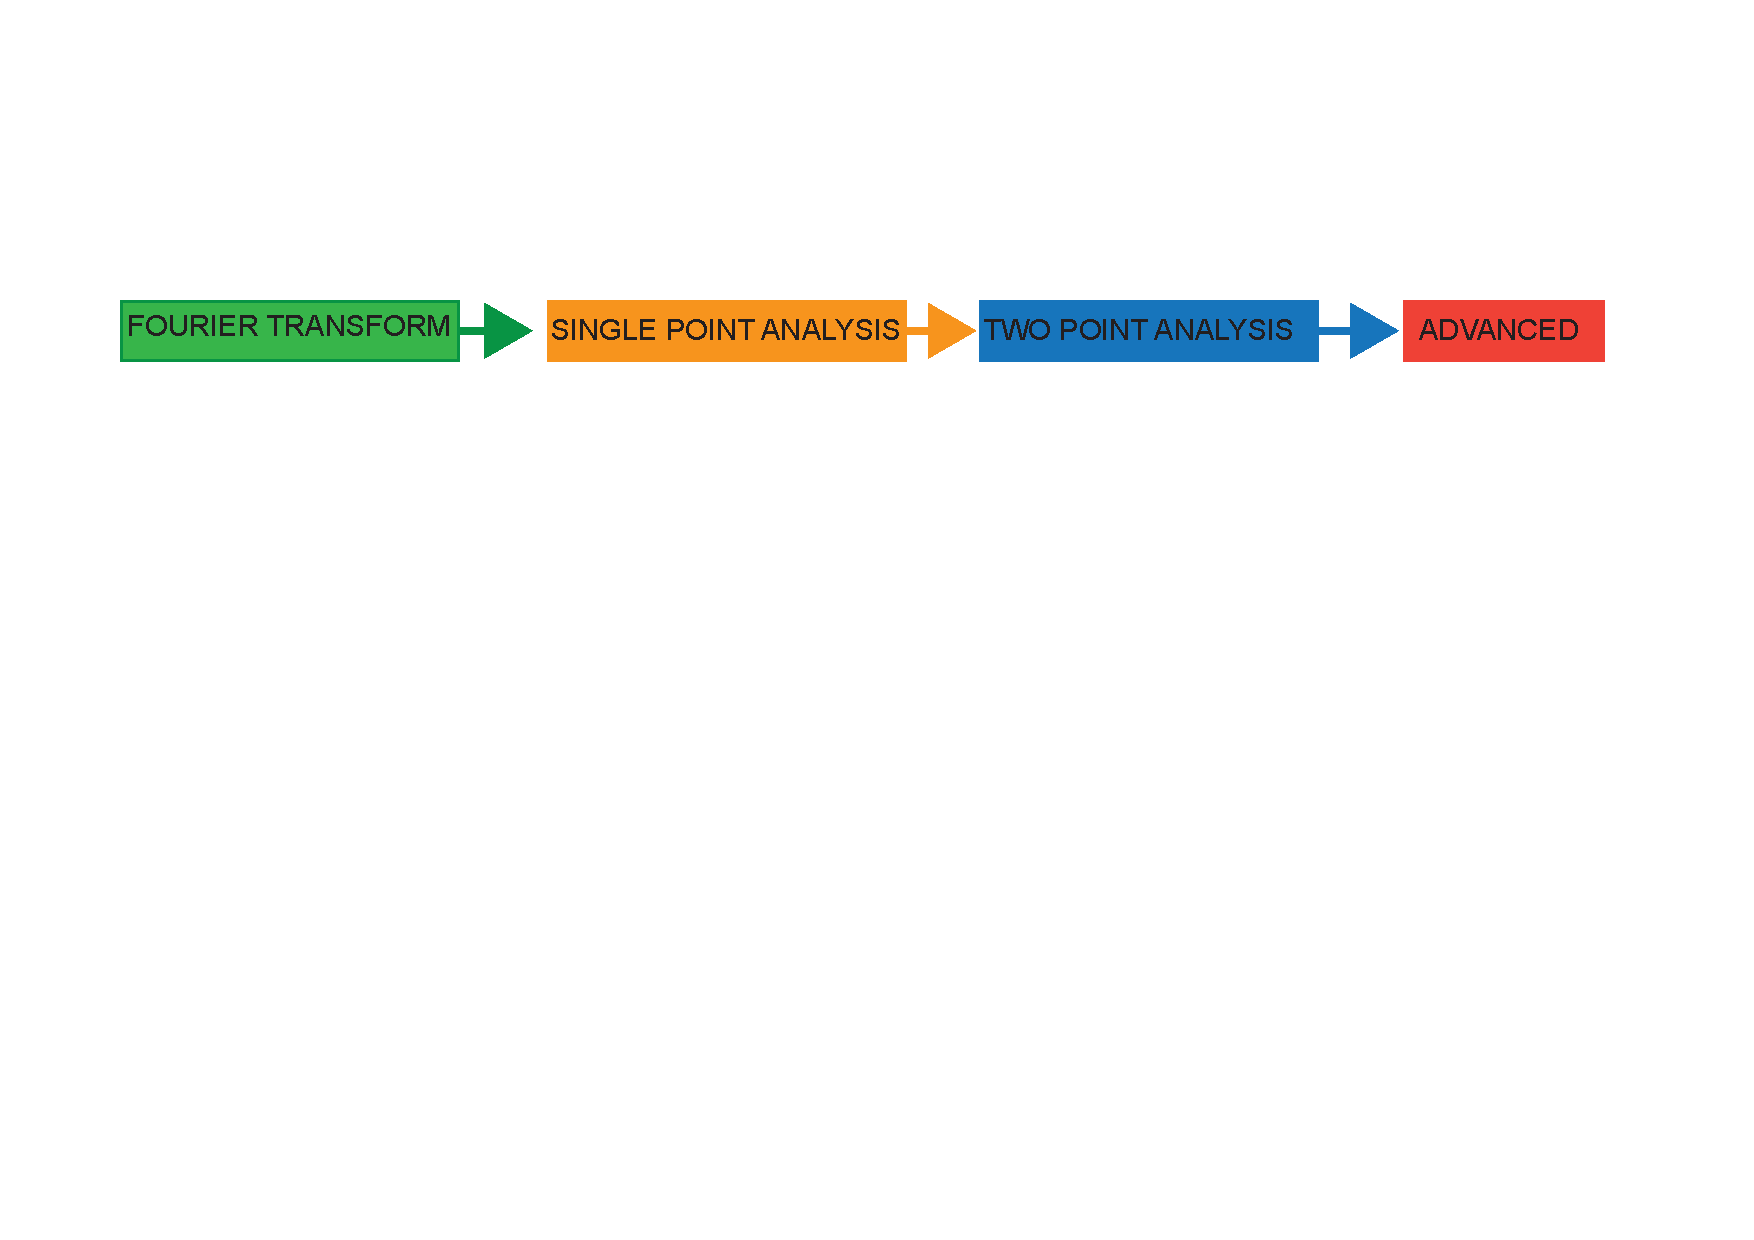
\includegraphics[width=\textwidth]{outline}
\end{center}}
\end{frame}

% \begin{frame}
% \frametitle{ The needs for the Fourier transform}
% %% per aggiungere la lettera colorata con l'argomento in alto a sx'
% \begin{tikzpicture}[remember picture, overlay]
% \node [shift={(-0.779 cm,-0.3cm)}]  at (current page.north east)
%    {\tikz[baseline=(t1.base)]{\node[fill=ta3chameleon](t1){%
% {\large A}};}
%     };
% \end{tikzpicture}
% %%
% \begin{itemize}[<+-|alert@+>]
% \item Generally theories are developed in the frequency/wavevector
%   domains ($\omega,\mathbf{k}$) rather than in time/space ($t,\mathbf{r}$)
% \item The reason for that resides principally on the fact that
%   \emph{Fourier transform} of governing equations allows an easier
%   treatment of typical mathematical operators
% \begin{equation*}
% \frac{\partial}{\partial t} \Longrightarrow i\omega; \qquad
% \frac{\partial f}{\partial x_i} \Longrightarrow i k_i \hat{f}(\mathbf{k},t)
% \end{equation*}
% \end{itemize}
% \onslide<3>{
% \begin{block}{}
% \begin{itemize}
% \item Some remarks on basic Fourier Transform and its discrete counterpart
% the Discrete Fourier Transform are mandatory
% \end{itemize}
% \end{block}
% }
% \end{frame}

\begin{frame}{Continuous and Discrete Fourier transform}
%% per aggiungere la lettera colorata con l'argomento in alto a sx'
\begin{tikzpicture}[remember picture, overlay]
\node [shift={(-0.779 cm,-0.3cm)}]  at (current page.north east)
   {\tikz[baseline=(t1.base)]{\node[fill=ta3chameleon](t1){%
{\large A}};}
    };
\end{tikzpicture}
%%

\begin{itemize}[<+->]
\item The \textcolor{taorange}{Direct} and \textcolor{cyan}{Inverse}
fourier transform of a generic function of time $x(t)$ is defined as :
{\small \begin{equation*}
\tikz[baseline=(t1.base)]{\node[fill=taorange](t1){%
$X(f) = \int_{-\infty}^{+\infty}x(t)e^{-2\pi i f t}\mathrm{d}t$};} \qquad
\tikz[baseline=(t1.base)]{\node[fill=cyan](t1){%
$x(t) = \int_{-\infty}^{+\infty}X(f)e^{2\pi i f t}\mathrm{d}f$};}
\end{equation*}}

\item In the case of discrete signals $x_n=x(n\Delta t)$ with $0\leq n
  \leq N-1$, sampled at frequency $f_c=\frac{1}{\Delta t}$ we have the
  corresponding \textcolor{taorange}{Direct} and \textcolor{cyan}{Inverse}
  Discrete Fourier transform 
{\small \begin{equation*}
\tikz[baseline=(t1.base)]{\node[fill=taorange](t1){%
$X_n = \frac{1}{N}\sum_{k=0}^{N-1}x_ke^{-2\pi kn/N}$};} \qquad
\tikz[baseline=(t1.base)]{\node[fill=cyan](t1){%
$x_k = \frac{1}{N}\sum_{n=-N/2}^{N/2}X_ne^{2\pi kn/N}$};}
\end{equation*}}

\only<3>{\item The \textcolor{ta3chameleon}{\texttt{Sampling Theorem}}
  {\footnotesize \parencite{Bracewell:1999ua}} ensure that 
\textcolor{rfxcyan}{a function whose
    Fourier transform is zero for $f>f_c$ is fully specified by values
  spaced at equal intervals not exceeding $\frac{1}{2}f_c^{-1}$}}
\only<4>{\item The \textcolor{ta3chameleon}{\texttt{Nyquist
      Frequency}} 
  $f_N = \frac{1}{2\Delta t}$, 
  defines the
  maximum frequency which can be properly resolved, or, equivalently,
  given the frequency of the system we would like to investigate, we
  had to sample at least at twice the values of this frequency.}
\end{itemize}
\end{frame}

\begin{frame}{Aliasing}
%% per aggiungere la lettera colorata con l'argomento in alto a sx'
\begin{tikzpicture}[remember picture, overlay]
\node [shift={(-0.779 cm,-0.3cm)}]  at (current page.north east)
   {\tikz[baseline=(t1.base)]{\node[fill=ta3chameleon](t1){%
{\large A}};}
    };
\end{tikzpicture}
%%

\begin{itemize}
\item The presence of frequency higher than the Nyquist frequency may
  lead to the presence of spurious frequency
\end{itemize}
\centering{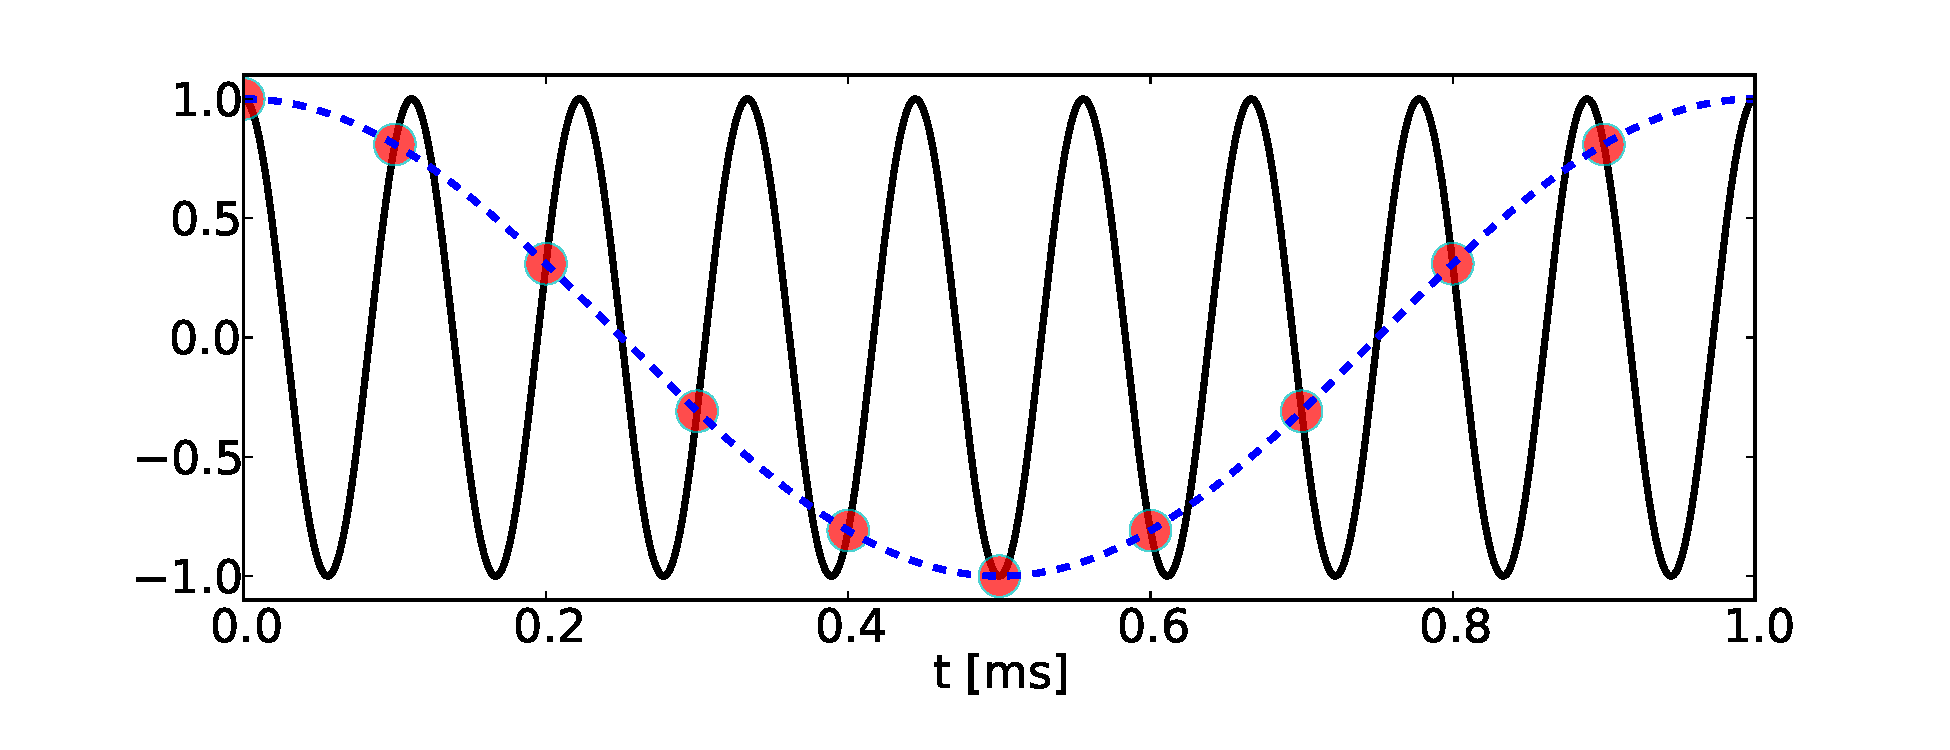
\includegraphics[height=4cm]{aliasing}}
\begin{itemize}
\item A 9 kHz cosine if sampled at 10 kHz exhibits a spurious 1 kHz oscillation
\end{itemize}
\end{frame}


\begin{frame}{Properties of Fourier transform}
%% per aggiungere la lettera colorata con l'argomento in alto a sx'
\begin{tikzpicture}[remember picture, overlay]
\node [shift={(-0.779 cm,-0.3cm)}]  at (current page.north east)
   {\tikz[baseline=(t1.base)]{\node[fill=ta3chameleon](t1){%
{\large A}};}
    };
\end{tikzpicture}
%%

\begin{itemize}
\item Various theorems may be applied to
  FT \parencite{Bracewell:1999ua} among which we cite:
\end{itemize}
% \only<2>{
\begin{theorem}{\underline{Convolution theorem:}}
If $x(t)$ and $g(t)$ have FT respectively equal to $X(f)$ and $G(f)$
the convolution of the two functions $h(t) = \int_{-\infty}^{+\infty}x(t^{'})g(t-t^{'})\mathrm{d}t^{'}$
is equal to $X(f)G(f)$
\end{theorem}
\begin{theorem}{\underline{Rayleigh's Theorem}}
The integral of squared modulus of a function is equal to the
integral of the squared modulus of its spectrum, i.e:
\begin{equation*}
\int_{-\infty}^{+\infty}|f(t)|^2\mathrm{d}t =
\int_{-\infty}^{+\infty}|F(f)|^2\mathrm{d}f
\end{equation*}
\end{theorem}
\end{frame}



\begin{frame}{Single Point: the autocorrelation function}
%% per aggiungere la lettera colorata con l'argomento in alto a sx'
\begin{tikzpicture}[remember picture, overlay]
\node [shift={(-0.779 cm,-0.3cm)}]  at (current page.north east)
   {\tikz[baseline=(t1.base)]{\node[fill=taorange](t1){%
{\large B}};}
    };
\end{tikzpicture}
%%

\begin{itemize}
\item A random process $x(t)$ is
  completely described by its moments, i.e. averages over the
  probability distribution function 
\begin{equation*}
E[x(t)] \quad
E[x(t_1)x(t_2)] \quad
E[x(t_1)x(t_2)x(t_3)] \quad
\ldots
\end{equation*}
\item We define the \textcolor{taskyblue}{\texttt{Auto-correlation function}}, i.e. 
  the second order momentum of the distribution, and the  
\textcolor{tachameleon}{\texttt{autocovariance
  function}}
{\small \begin{equation*}
\tikz[baseline=(t1.base)]{\node[fill=taskyblue](t1){%
$R(\tau)= E|x(t)x(t-\tau)|$};} \qquad
\tikz[baseline=(t1.base)]{\node[fill=tachameleon](t1){%
$C(\tau) = E|(x(t)-m)(x(t-\tau)-m)|$};}
\end{equation*}}
being $m$ the average of $x(t)$
\item The \textcolor{ta3orange}{\texttt{Auto-correlation coefficient factor}}
  is defined as $\rho(\tau)=C(\tau)/C(0)$
\item For digitized signals with $N$ samples the estimator of
  $C(\tau)$ is defined as 
{\small \begin{equation*}
C_j =
\frac{1}{N}\sum_{i=j}^{N-1}(x_i-\overline{x})(x_{i-j}-\overline{x})
\qquad \overline{x}=\frac{1}{N}\sum_{i=0}^{N-1}x_i
\end{equation*}}
\end{itemize}
\end{frame}

\begin{frame}{Auto-correlation: practical use}
%% per aggiungere la lettera colorata con l'argomento in alto a sx'
\begin{tikzpicture}[remember picture, overlay]
\node [shift={(-0.779 cm,-0.3cm)}]  at (current page.north east)
   {\tikz[baseline=(t1.base)]{\node[fill=taorange](t1){%
{\large B}};}
    };
\end{tikzpicture}
%%
\begin{itemize}
\item Define the \textcolor{ta3chameleon}{\texttt{Auto-correlation time}} of
  a turbulent field such as the potential: $R(\tau_c)=\frac{\text{max}(R(\tau))}{e}$

\begin{center}
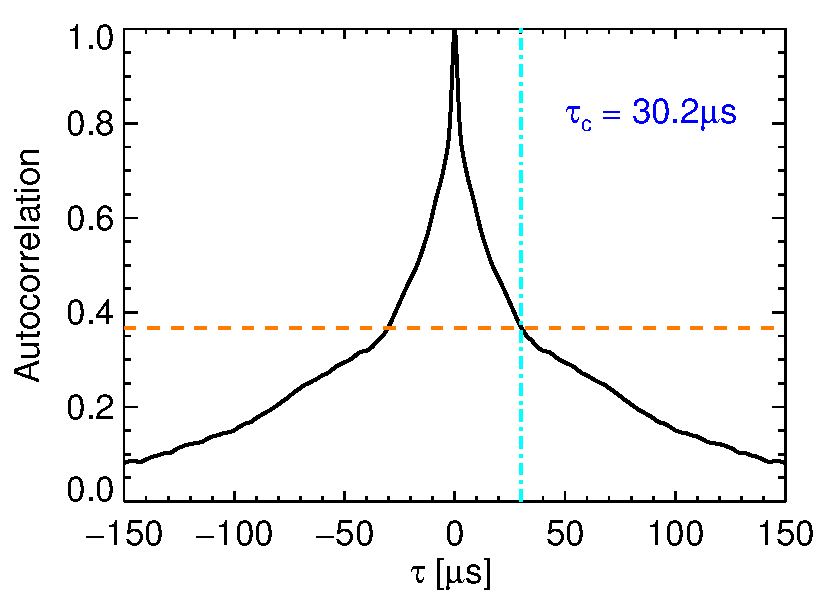
\includegraphics[height=5cm]{Auto-correlation20367}
\end{center}

\end{itemize}
\end{frame}

\begin{frame}{Single point: the power spectrum}
%% per aggiungere la lettera colorata con l'argomento in alto a sx'
\begin{tikzpicture}[remember picture, overlay]
\node [shift={(-0.779 cm,-0.3cm)}]  at (current page.north east)
   {\tikz[baseline=(t1.base)]{\node[fill=taorange](t1){%
{\large B}};}
    };
\end{tikzpicture}
%%
\begin{itemize}[<+->]
\item The \textcolor{ta3skyblue}{Power spectrum $S(f)$} is defined as the
  Fourier transform of the Autocorrelation-function.
\item It describes the frequency distribution of the \emph{power of
    the signal.} 
\item It corresponds to the limit of the
  \textcolor{ta3skyblue}{\texttt{periodogram}}  of limited signals $x_T(t)$
 $\frac{E[FT(x_T(t)) ^2]}{T}\xrightarrow[T\rightarrow \infty]{} S(f)$
\item Numerically, the signal is divided into $M$ slices, treated as
  independent realizations, and we compute the power spectral estimator $\hat{S}_n$
 related to the real power spectrum $S(f_n)$ according to
\begin{equation*}
\hat{S}_n = \frac{1}{M}\sum_{k=1}^{M}|X_n^{(k)}|^2; \qquad \hat{S}_n
\simeq S(f_n)\Delta f
\end{equation*}
\end{itemize}
\end{frame}

\begin{frame}{Power spectrum: practical use}
%% per aggiungere la lettera colorata con l'argomento in alto a sx'
\begin{tikzpicture}[remember picture, overlay]
\node [shift={(-0.779 cm,-0.3cm)}]  at (current page.north east)
   {\tikz[baseline=(t1.base)]{\node[fill=taorange](t1){%
{\large B}};}
    };
\end{tikzpicture}
%%
\only<1-2>{\begin{columns}[c]
\begin{column}{.4\textwidth}
\begin{itemize}
{\small \item \textcolor{ta3scarletred}{Mode identification at a given
    frequency {\footnotesize \parencite{Conway:2005gq}}}}
\end{itemize}
\end{column}
\begin{column}{0.6\textwidth}
\centering{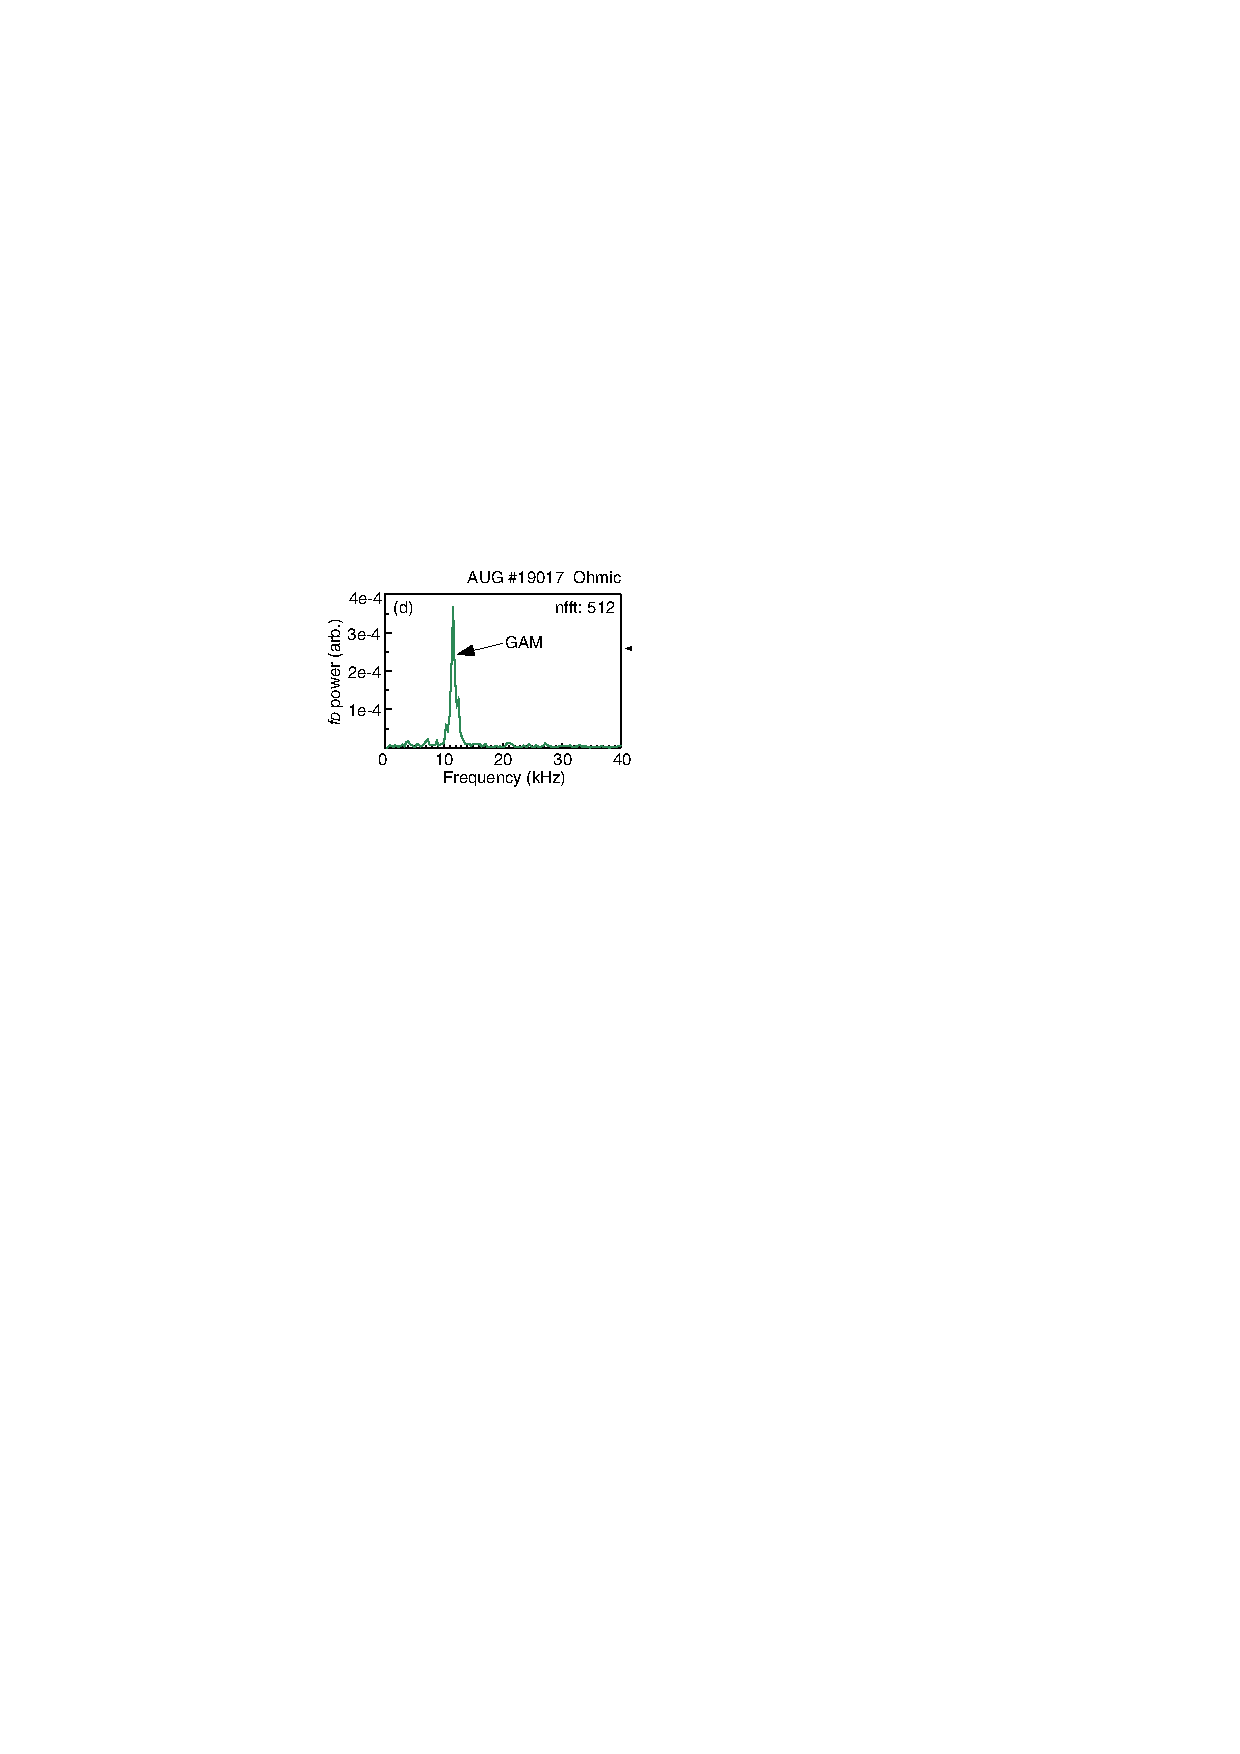
\includegraphics[width=0.67\textwidth]{gam-conway}}
%{\footnotesize G. Conway PPCF }
\end{column}
\end{columns}
}
\only<2>{\begin{columns}[c]
\begin{column}{0.6\textwidth}
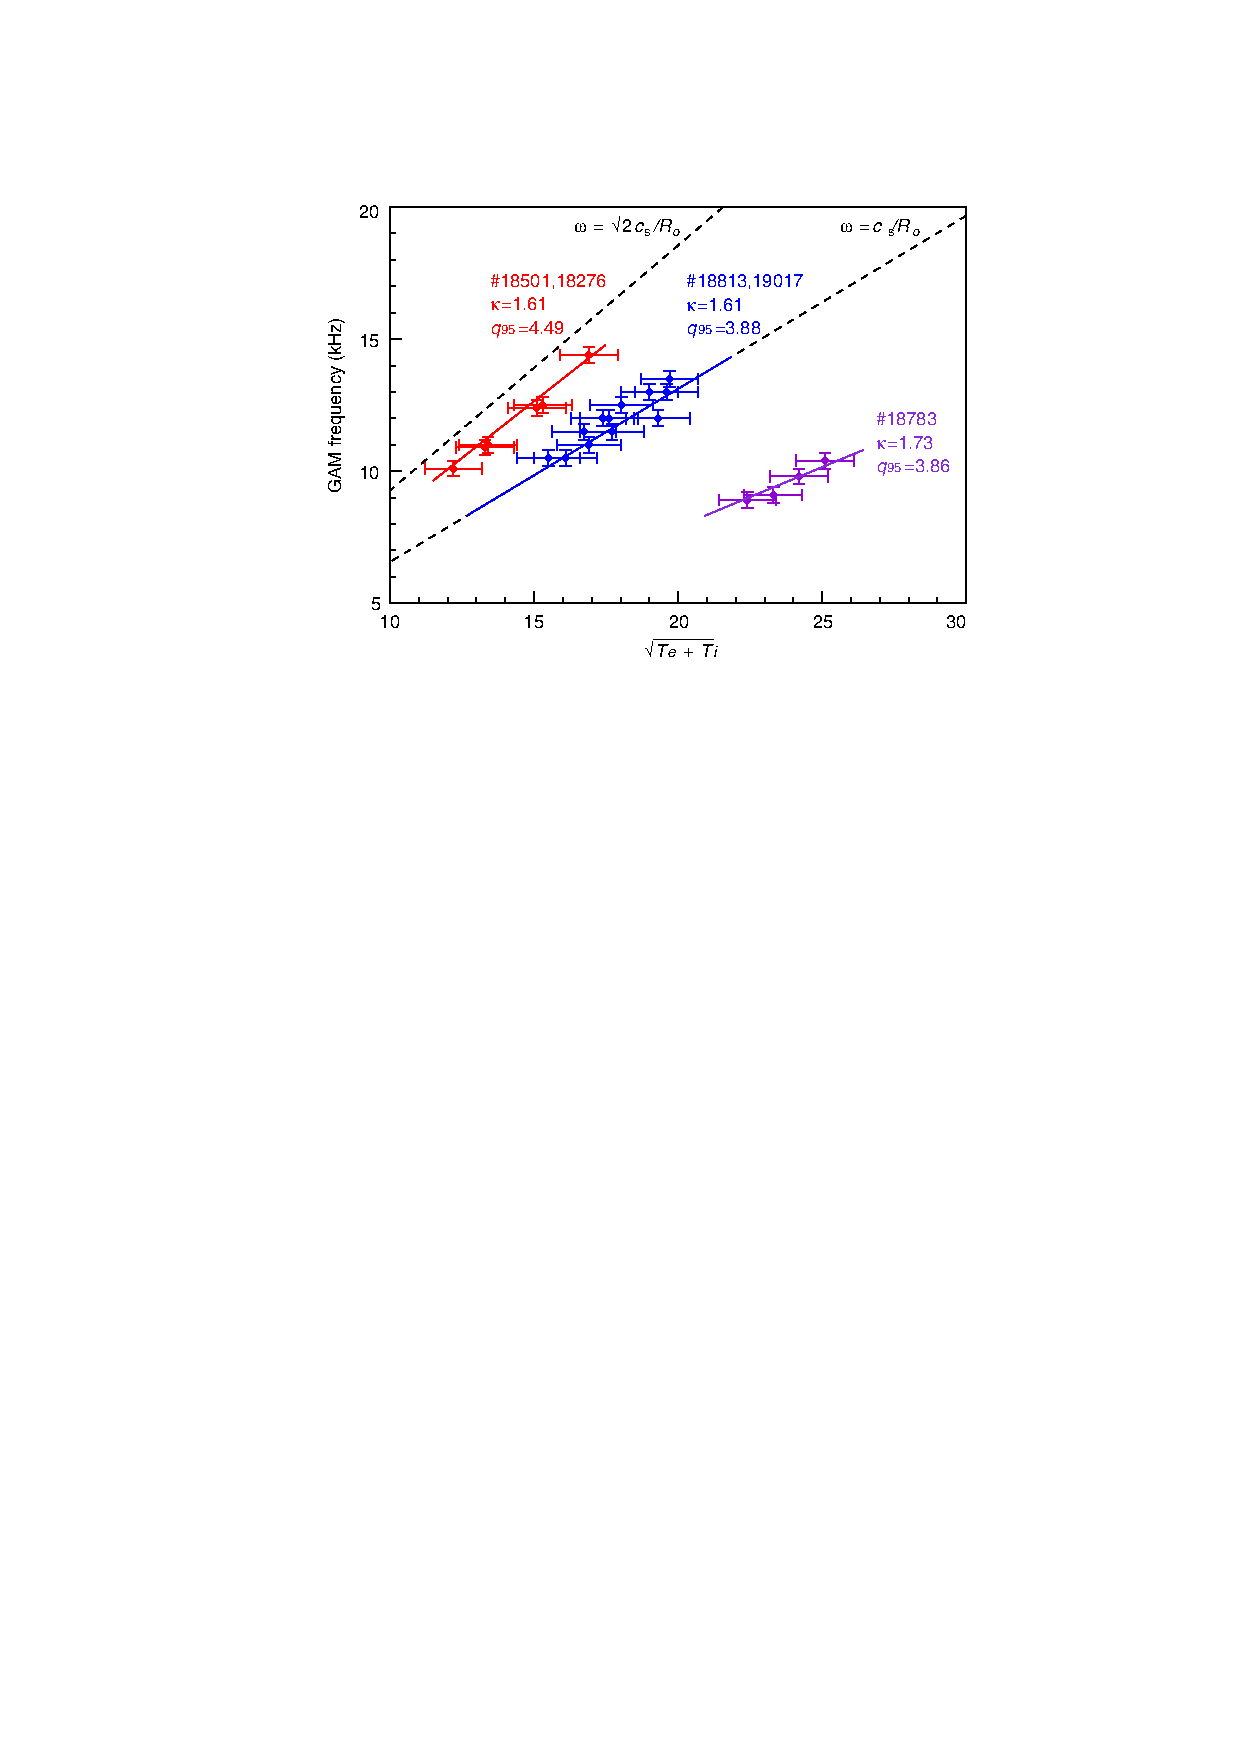
\includegraphics[width=6.cm]{gam-scaling}
\end{column}
\begin{column}{0.4\textwidth}
{\small \begin{itemize}
\item Information must be completed. In the
  example \textcolor{taskyblue}{Geodesic Acoustic Modes} identified
  considering their scaling with $c_s$
\end{itemize}}
\end{column}
\end{columns}
}\end{frame}

\begin{frame}{Power spectrum: The spectrogram}
%% per aggiungere la lettera colorata con l'argomento in alto a sx'
\begin{tikzpicture}[remember picture, overlay]
\node [shift={(-0.779 cm,-0.3cm)}]  at (current page.north east)
   {\tikz[baseline=(t1.base)]{\node[fill=taorange](t1){%
{\large B}};}
    };
\end{tikzpicture}
%%
\begin{itemize}
{\footnotesize \item The same information can be also analyzed in time applying the
  \textcolor{tascarletred}{\texttt{spectrogram}} technique in the time/frequency
  space {\footnotesize \parencite{spagnolo}}
}

\begin{center}
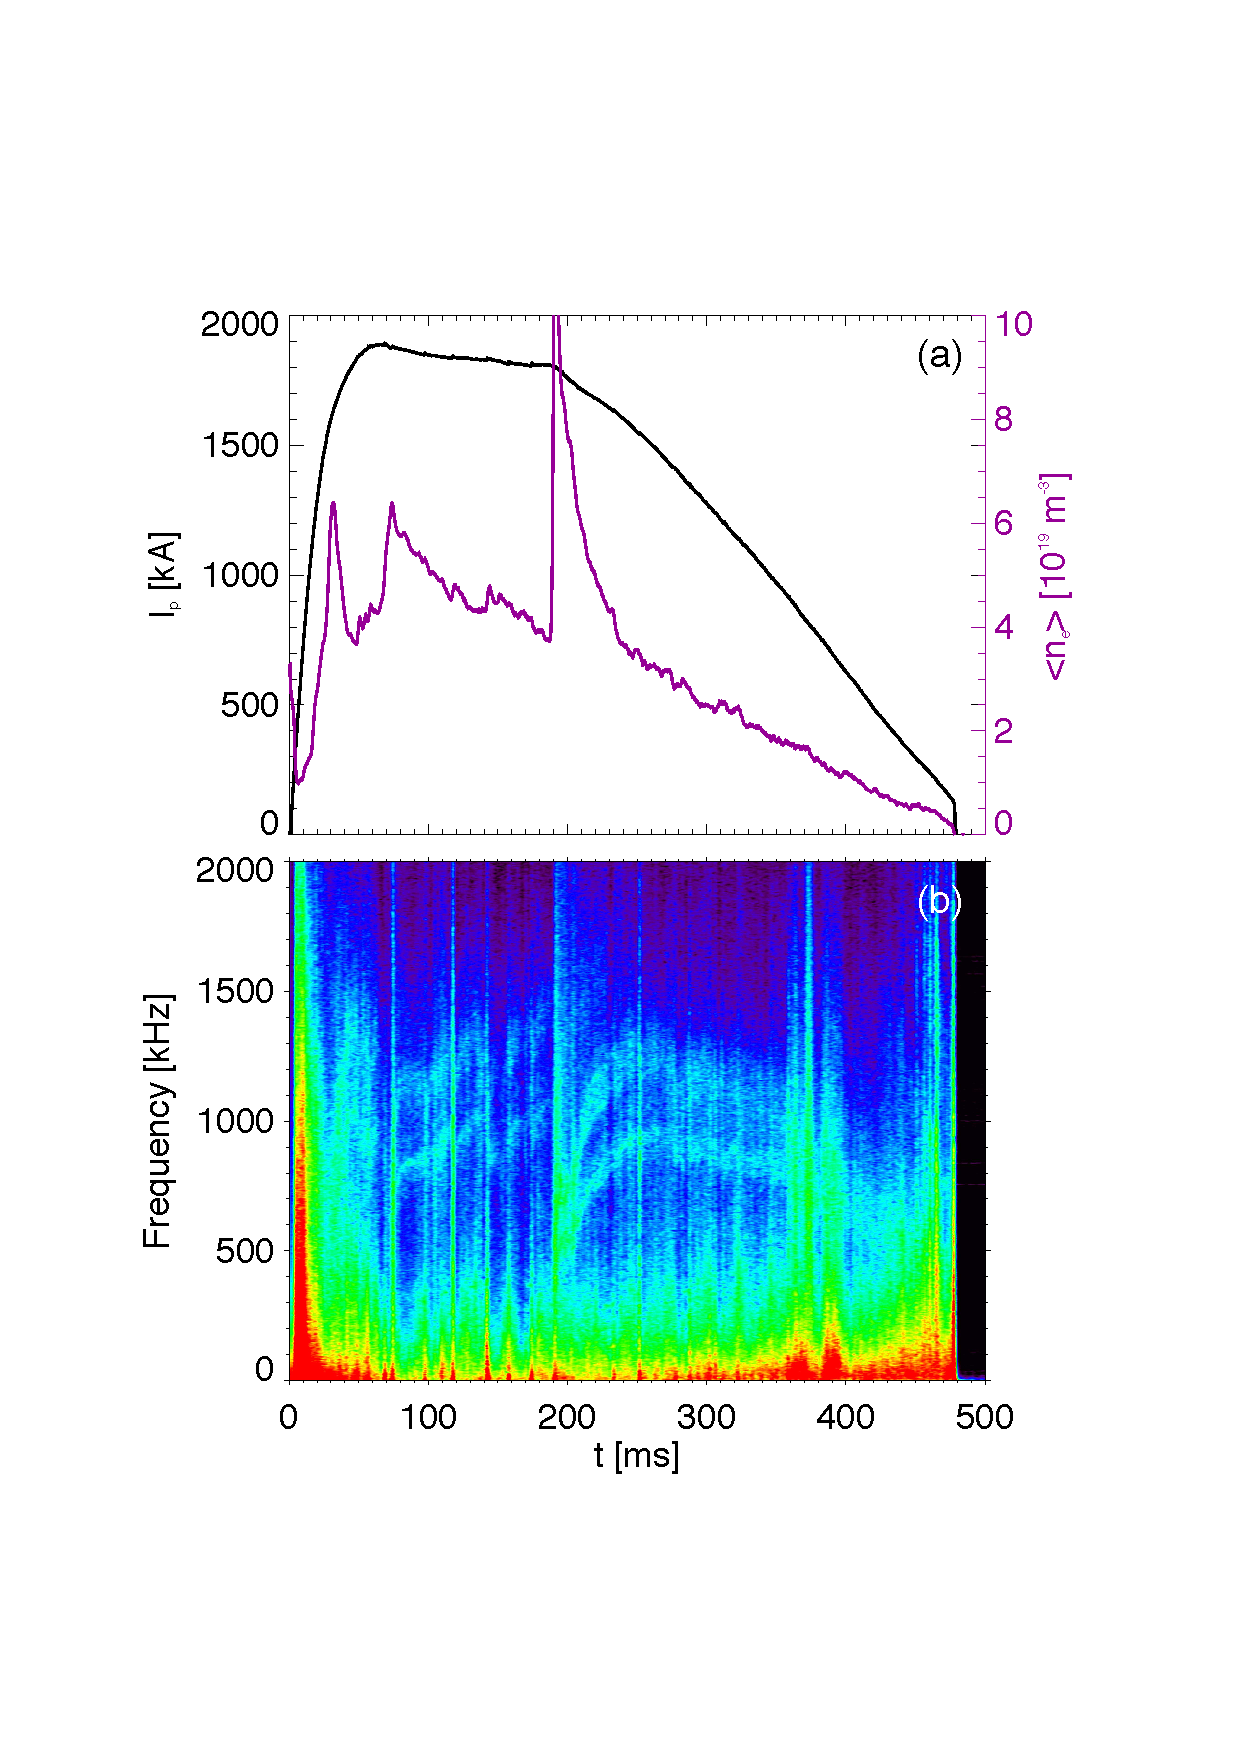
\includegraphics[height=5.cm]{alfven} 
\end{center}
{\footnotesize\item Alfv\'enic nature, with $\omega$ dependent from the
  Alfv\'en velocity $v_A = B/\sqrt{\rho\mu_0}$, revealed by the
  comparison with the plasma density
}\end{itemize}
\end{frame}


\begin{frame}{Two-points techniques}
%% per aggiungere la lettera colorata con l'argomento in alto a sx'
\begin{tikzpicture}[remember picture, overlay]
\node [shift={(-0.779 cm,-0.3cm)}]  at (current page.north east)
   {\tikz[baseline=(t1.base)]{\node[fill=ta2skyblue](t1){%
{\large C}};}
    };
\end{tikzpicture}
%%
\begin{itemize}[<+->]
\item Spatially distributed measurements allow access to spatial
  structure of the fluctuations
\item The minimum set includes two measurements $x(t)$ and $y(t)$. We can define the
  \textcolor{tascarletred}{\texttt{Cross-correlation function}},
  \textcolor{taorange}{\texttt{The cross-covariance function}} and the
  \textcolor{taskyblue}{\texttt{cross-correlation coefficient function}}
{\footnotesize \begin{gather*}
\tikz[baseline=(t1.base)]{\node[fill=tascarletred](t1){%
$R_{xt}(\tau)=E[y(t)x(t-\tau)]$};}  \\
\tikz[baseline=(t1.base)]{\node[fill=taorange](t1){%
$C_{xy}(\tau)=E[(y(t)-\overline{y})(x(t-\tau)-\overline{x})]$};} \\
\tikz[baseline=(t1.base)]{\node[fill=taskyblue](t1){%
$\rho_{yx}(\tau) = \frac{C_{yx}(\tau)}{\sqrt{C_{xx}(0)C_{yy}(0)}}$};}
\end{gather*}}
\item The discrete counterpart of the cross-covariance is
  defined as
{\footnotesize\begin{equation*}
C_{yx,j}=\frac{1}{N}\sum_{i=j}^{N-1}(y_i-\overline{y})(x_{i-j}-\overline{x})
\end{equation*}
}
\end{itemize}
\end{frame}

\begin{frame}{Two-points technique}
%% per aggiungere la lettera colorata con l'argomento in alto a sx'
\begin{tikzpicture}[remember picture, overlay]
\node [shift={(-0.779 cm,-0.3cm)}]  at (current page.north east)
   {\tikz[baseline=(t1.base)]{\node[fill=ta2skyblue](t1){%
{\large C}};}
    };
\end{tikzpicture}
%%
\begin{itemize}[<+->]
\item In analogy to the power spectrum we define the
  \textcolor{tascarletred}{Cross-power spectrum $S_{XY}(f)$} as the
  Fourier transform of the cross-correlation function
\item If $x(t)$ and $y(t)$ are real
  function, the cross-power spectrum is totally defined by the
  positive frequency only
\item The cross-spectrum is
  complex-valued $S_{YX}(f)=|S_{YX}(f)|e^{i\Theta_{YX}(f)}$ with
  $\Theta_{YX}(f)$ equal to the \textcolor{tascarletred}{\texttt{Phase
    spectrum}}
\item We define the
  \textcolor{tascarletred}{\texttt{coherence}} as $\gamma_{YX}(f)=\frac{|S_{YX}(f)|}{\sqrt{S_Y(f)S_X(f)}}$
\item In the case of discrete signals with finite temporal length the following definitions hold
  (in analogy to single point case)
\begin{equation*}
\hat{S}_{Y,X,n}= \frac{1}{M}\sum_{k=1}^MY_n^{(k)}X_n^{*(k)} \qquad
\hat{S}_{Y,X,n}\simeq S_{YX}(f_n)\Delta f
\end{equation*}
\end{itemize}
\end{frame}

\begin{frame}{Phase spectrum}
%% per aggiungere la lettera colorata con l'argomento in alto a sx'
\begin{tikzpicture}[remember picture, overlay]
\node [shift={(-0.779 cm,-0.3cm)}]  at (current page.north east)
   {\tikz[baseline=(t1.base)]{\node[fill=ta2skyblue](t1){%
{\large C}};}
    };
\end{tikzpicture}
%%
\begin{itemize}[<+->]
\item The method can be applied also in the case of two quantities
  measured on the same location
\item In the case of Langmuir probes for example, electron density
  $n_e$ and plasma potential $\phi_p$ are know in the same nominal
  position

\centering{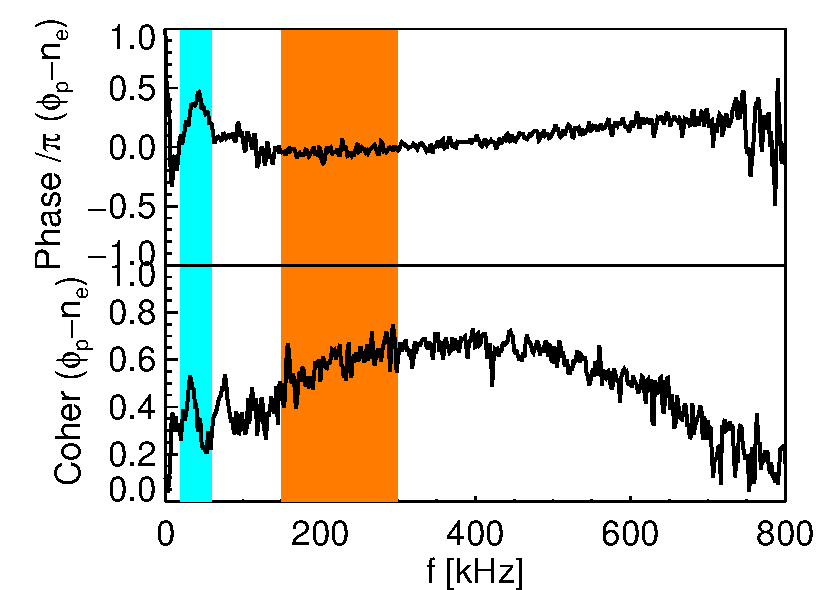
\includegraphics[height=3.88cm]{PhaseCoherenceEn-Vp20367}}

\item This allow the possibility to distinguish the frequency where
  turbulence is \textcolor{rfxcyan}{Interchange-dominated} from that
  where turbulence is \textcolor{orange}{Drift-dominated}
% \item Other possibility is the determination of the polarization of
%   magnetic fluctuations frequency resolved 
\end{itemize}
\end{frame}

\begin{frame}{Wave-vector estimate}
%% per aggiungere la lettera colorata con l'argomento in alto a sx'
\begin{tikzpicture}[remember picture, overlay]
\node [shift={(-0.779 cm,-0.3cm)}]  at (current page.north east)
   {\tikz[baseline=(t1.base)]{\node[fill=ta2skyblue](t1){%
{\large C}};}
    };
\end{tikzpicture}
%%
\begin{itemize}[<+->]
\item In the case of a reasonably deterministic dispersion relation between $k$ and $f$, the phase may be
  used for the determination of $k$
\item\textcolor{ta3chameleon}{\texttt{Wave vector}} is
  estimated from \textcolor{ta3chameleon}{\texttt{Phase spectrum}}
\begin{center}
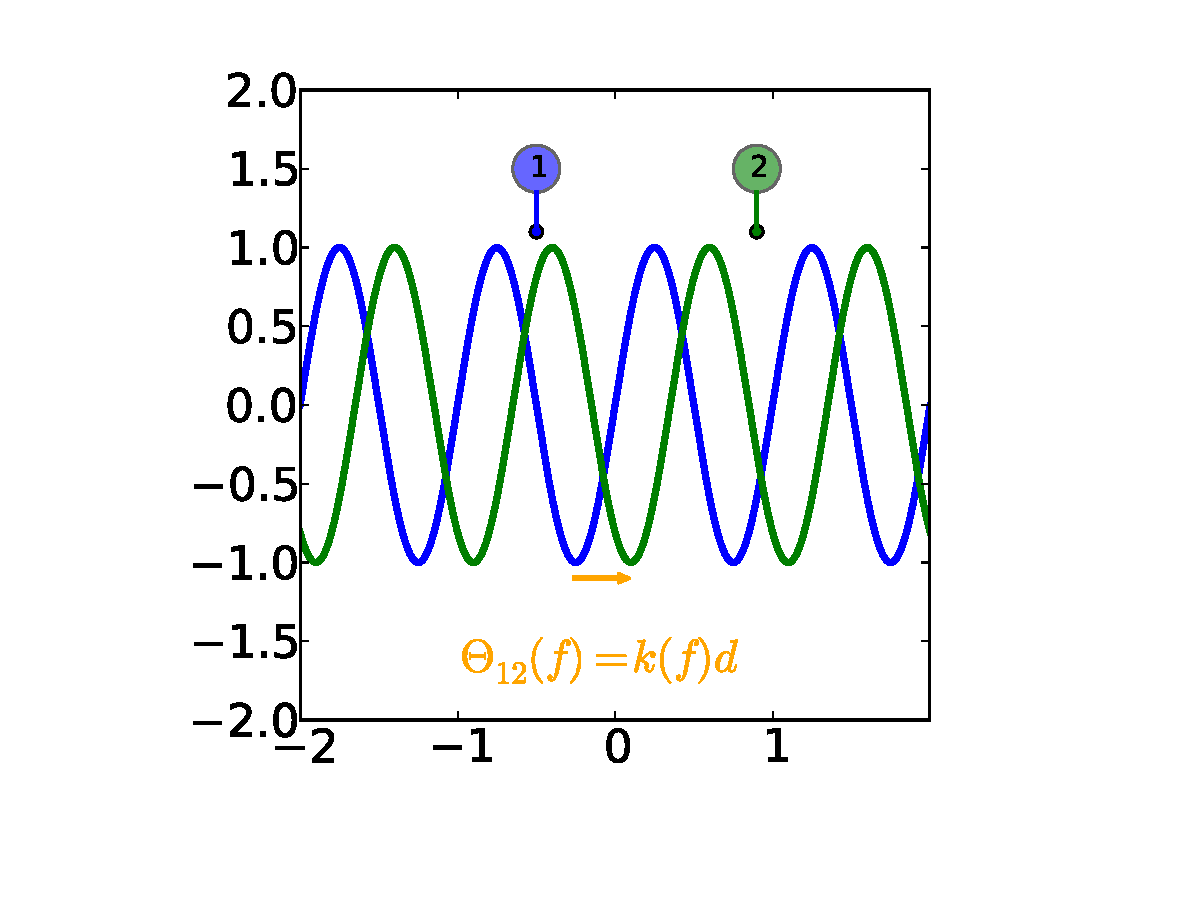
\includegraphics[height=4cm]{phase-shift}
\end{center}
\item \textcolor{tachameleon}{Distance $d$ must be less than
  a wave length, less than a correlation length, but far enough the
  detect a measurable phase difference}
\end{itemize}
\end{frame}

\begin{frame}{Fluctuation-induced particle transport}
%% per aggiungere la lettera colorata con l'argomento in alto a sx'
\begin{tikzpicture}[remember picture, overlay]
\node [shift={(-0.779 cm,-0.3cm)}]  at (current page.north east)
   {\tikz[baseline=(t1.base)]{\node[fill=ta2skyblue](t1){%
{\large C}};}
    };
\end{tikzpicture}
%%
\begin{itemize}
\item Fluctuations induced particle flux is defined as $\Gamma = E[\tilde{n}(t)\tilde{v}(t)]=E[\tilde{n}(t)\tilde{E}(t)]/B$
\item According to previous definitions and properties 
\begin{equation*}
\Gamma
=\frac{1}{B}R_{nE}(\tau=0)= \frac{2}{B}\int_0^{+\infty}\Re[S_{nE}(f)]df
\end{equation*}
\item In quasi-static approximation $\tilde{E}=-\nabla\tilde{\phi}$,
  with finite record length $T$, and assuming a deterministic
  dispersion relation 
\begin{equation*}
\Gamma(f)=\frac{2k(f)}{B}\Im\{S_{n\phi}(f)\} 
\end{equation*}
\end{itemize}
\end{frame}

\begin{frame}{Fluctuation-induced particle transport 2}
%% per aggiungere la lettera colorata con l'argomento in alto a sx'
\begin{tikzpicture}[remember picture, overlay]
\node [shift={(-0.779 cm,-0.3cm)}]  at (current page.north east)
   {\tikz[baseline=(t1.base)]{\node[fill=ta2skyblue](t1){%
{\large C}};}
    };
\end{tikzpicture}
%%
\begin{itemize}
{\footnotesize
\item In practice, considering digitized signals we have
  \footnotesize{(see for example \parencite{Antoni:2000bn})}
\begin{equation*}
\Gamma(f)=\frac{1}{M}\sum_{k=1}^{M}\Gamma^{k}(f) = \frac{2}{BM}\sum_{k=1}^{M-1}\Im\{k^{(k)}(f)N^{(k)}(f)\Phi^{*(k)}(f)\}
\end{equation*}
}
\only<2>{
\centering{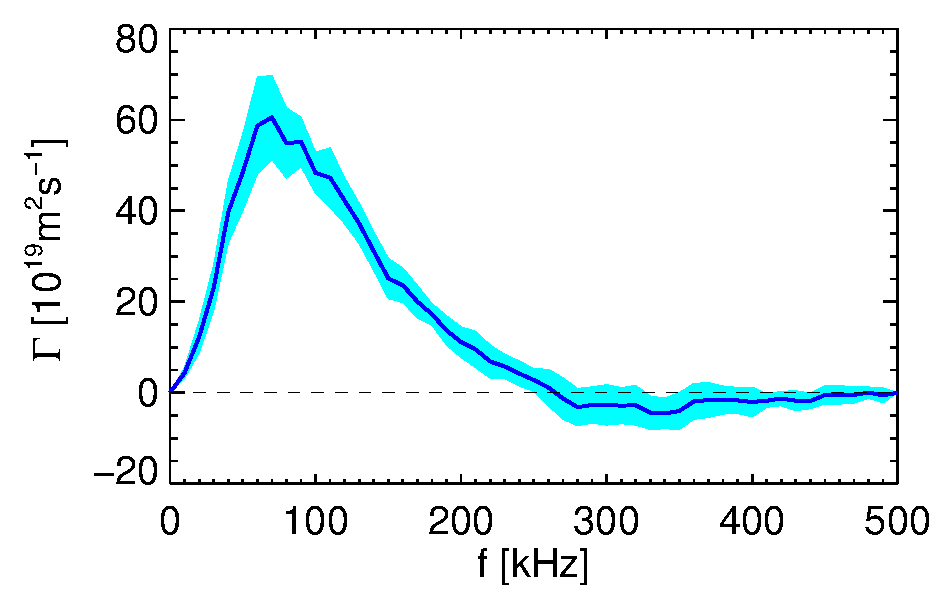
\includegraphics[height=3.5cm]{flux_vs_f}}
}

\only<3>{
\centering{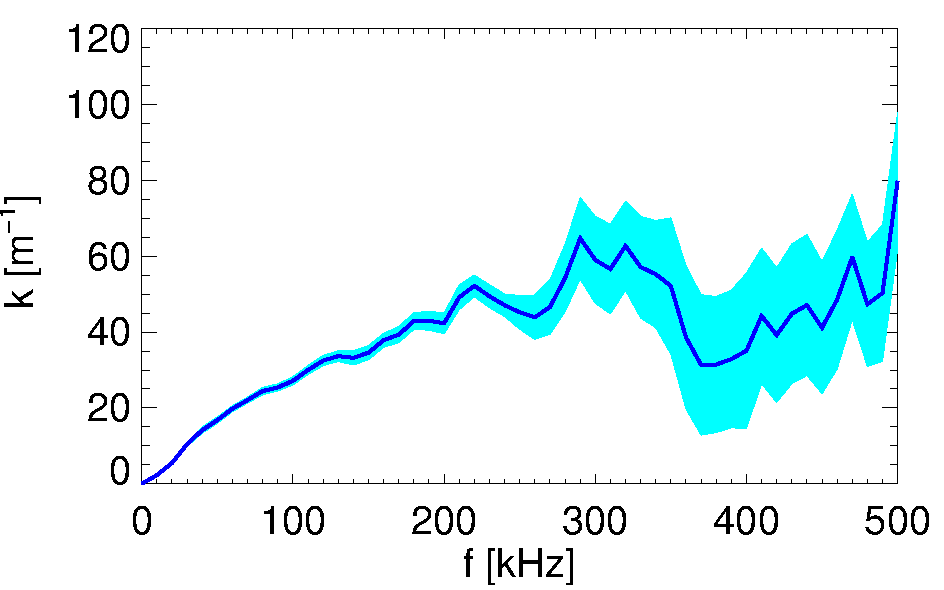
\includegraphics[height=3.5cm]{k_vs_f}}
}

\only<4>{
\centering{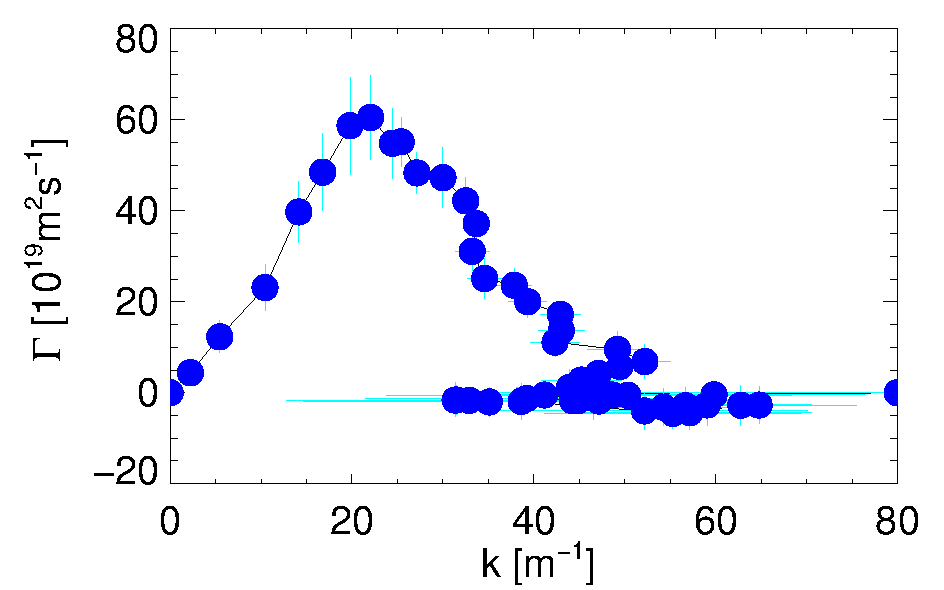
\includegraphics[height=3.5cm]{flux_vs_k}}
}
\end{itemize}
\end{frame}


\begin{frame}{More than transport of particles}
%% per aggiungere la lettera colorata con l'argomento in alto a sx'
\begin{tikzpicture}[remember picture, overlay]
\node [shift={(-0.779 cm,-0.3cm)}]  at (current page.north east)
   {\tikz[baseline=(t1.base)]{\node[fill=ta2skyblue](t1){%
{\large C}};}
    };
\end{tikzpicture}
%%
\begin{itemize}
\item Similar method may be used for the determination of the
  \emph{Reynolds stress} $\langle\tilde{v}_r\tilde{v}_{\perp}\rangle$
  which play a role in the momentum generation for both Tokamak and
  RFPs as $\partial_t(V_{\phi}) \propto
  -\partial_r\langle\tilde{v}_r\tilde{v}_{\phi}\rangle + \ldots$ {\footnotesize
  (see e.g. \parencite{Vianello:2005hf,Vianello:2005dt,Vianello:2006bn})}
\end{itemize}
\begin{center}
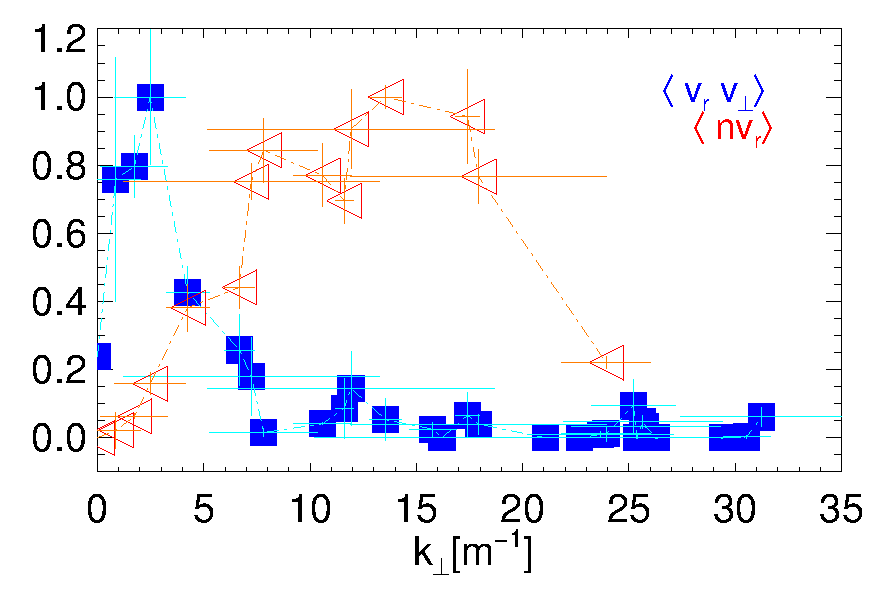
\includegraphics[height=4cm]{ErsFlux_vsk}
\end{center}

\end{frame}


\begin{frame}{The wavenumber-frequency Spectrum}
%% per aggiungere la lettera colorata con l'argomento in alto a sx'
\begin{tikzpicture}[remember picture, overlay]
\node [shift={(-0.779 cm,-0.3cm)}]  at (current page.north east)
   {\tikz[baseline=(t1.base)]{\node[fill=ta2skyblue](t1){%
{\large C}};}
    };
\end{tikzpicture}
%%
\begin{itemize}[<+->]
\item For turbulent medium, with different wave
  numbers corresponding to the same frequency we need to compute the \textcolor{tachameleon}{\texttt{Wave
      number-frequency power spectrum $S(k,\omega)$}}
\item This is equivalent to the Fourier transform of the space time
  correlation function $R(\chi,\tau)$
\begin{equation*}
S(k,\omega)
=\iint_{-\infty}^{+\infty}R(\chi,\tau)e^{-i(\omega\tau-k\chi)}d\chi d\tau
\end{equation*}
\item In the two 2 points cases are available, the spectrum is
  reconstructed on a statistical basis considering the $M$ different realizations:
{\small\begin{gather*}
\hat{S}_L(k,\omega)=\hat{S}_L(p\Delta k,2\pi n \Delta
f)=\frac{1}{M}\sum_{j=1}^M S_n^{(j)}I_p[k_n^{j}] \\ 
I_p[k_n^{j}] = 
\begin{cases}
1 \;\text{for}\; (p-1/2)\Delta k < k_n^{(j)}< (p+1/2)\Delta k \\
0 \;\text{elsewhere}
\end{cases}
\end{gather*}}


\end{itemize}

\end{frame}

\begin{frame}{Spectral power density}
%% per aggiungere la lettera colorata con l'argomento in alto a sx'
\begin{tikzpicture}[remember picture, overlay]
\node [shift={(-0.779 cm,-0.3cm)}]  at (current page.north east)
   {\tikz[baseline=(t1.base)]{\node[fill=ta2skyblue](t1){%
{\large C}};}
    };
\end{tikzpicture}
%%


\only<1>{
\begin{itemize}
\item Spectral power density from GPI LoS on NSTX {\footnotesize\parencite{Agostini:2007kx}}

\vspace{1cm}

\centering{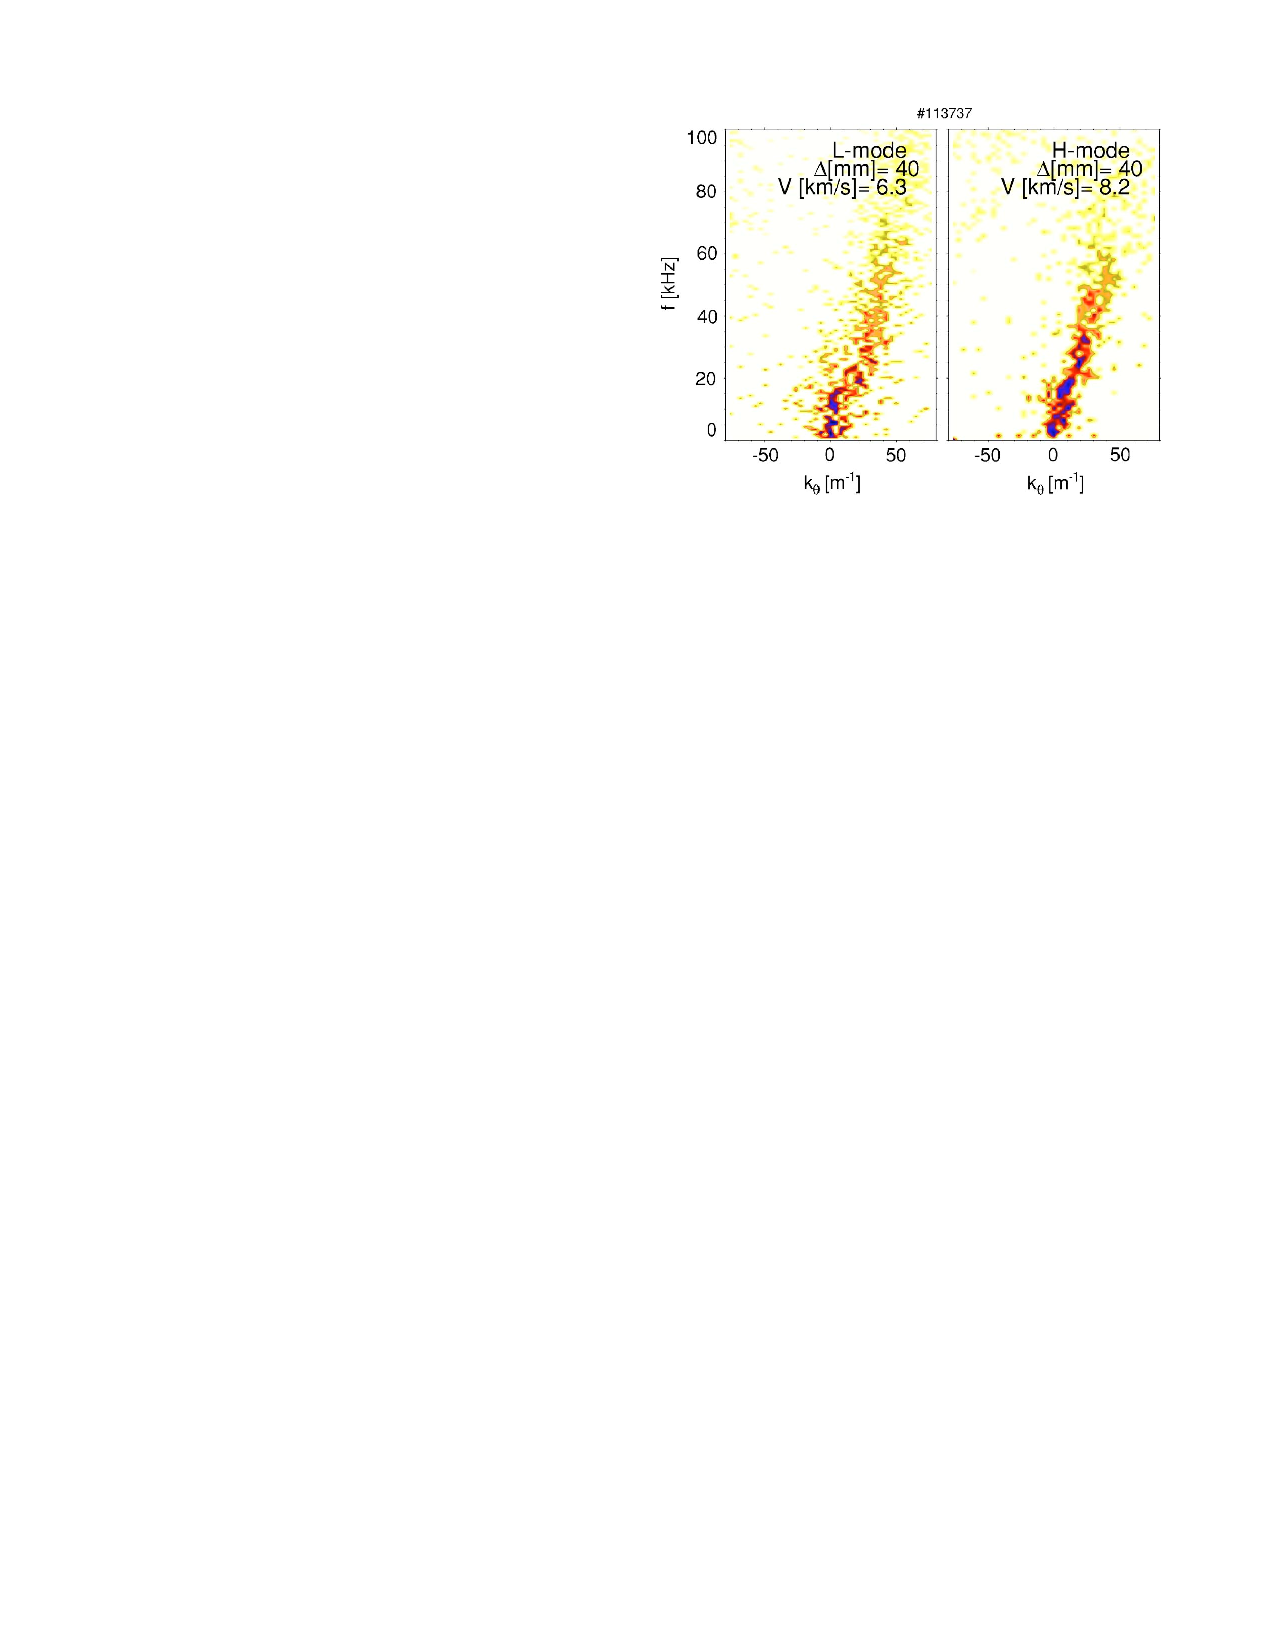
\includegraphics[height=4.5cm]{skf}}
\end{itemize}
}

\only<2>{
\begin{itemize}
\item We can consequently compute
  $S(k)=\int_{-\infty}^{+\infty}S(k,\omega)\frac{d\omega}{2\pi}$

\vspace{1cm}

\centering{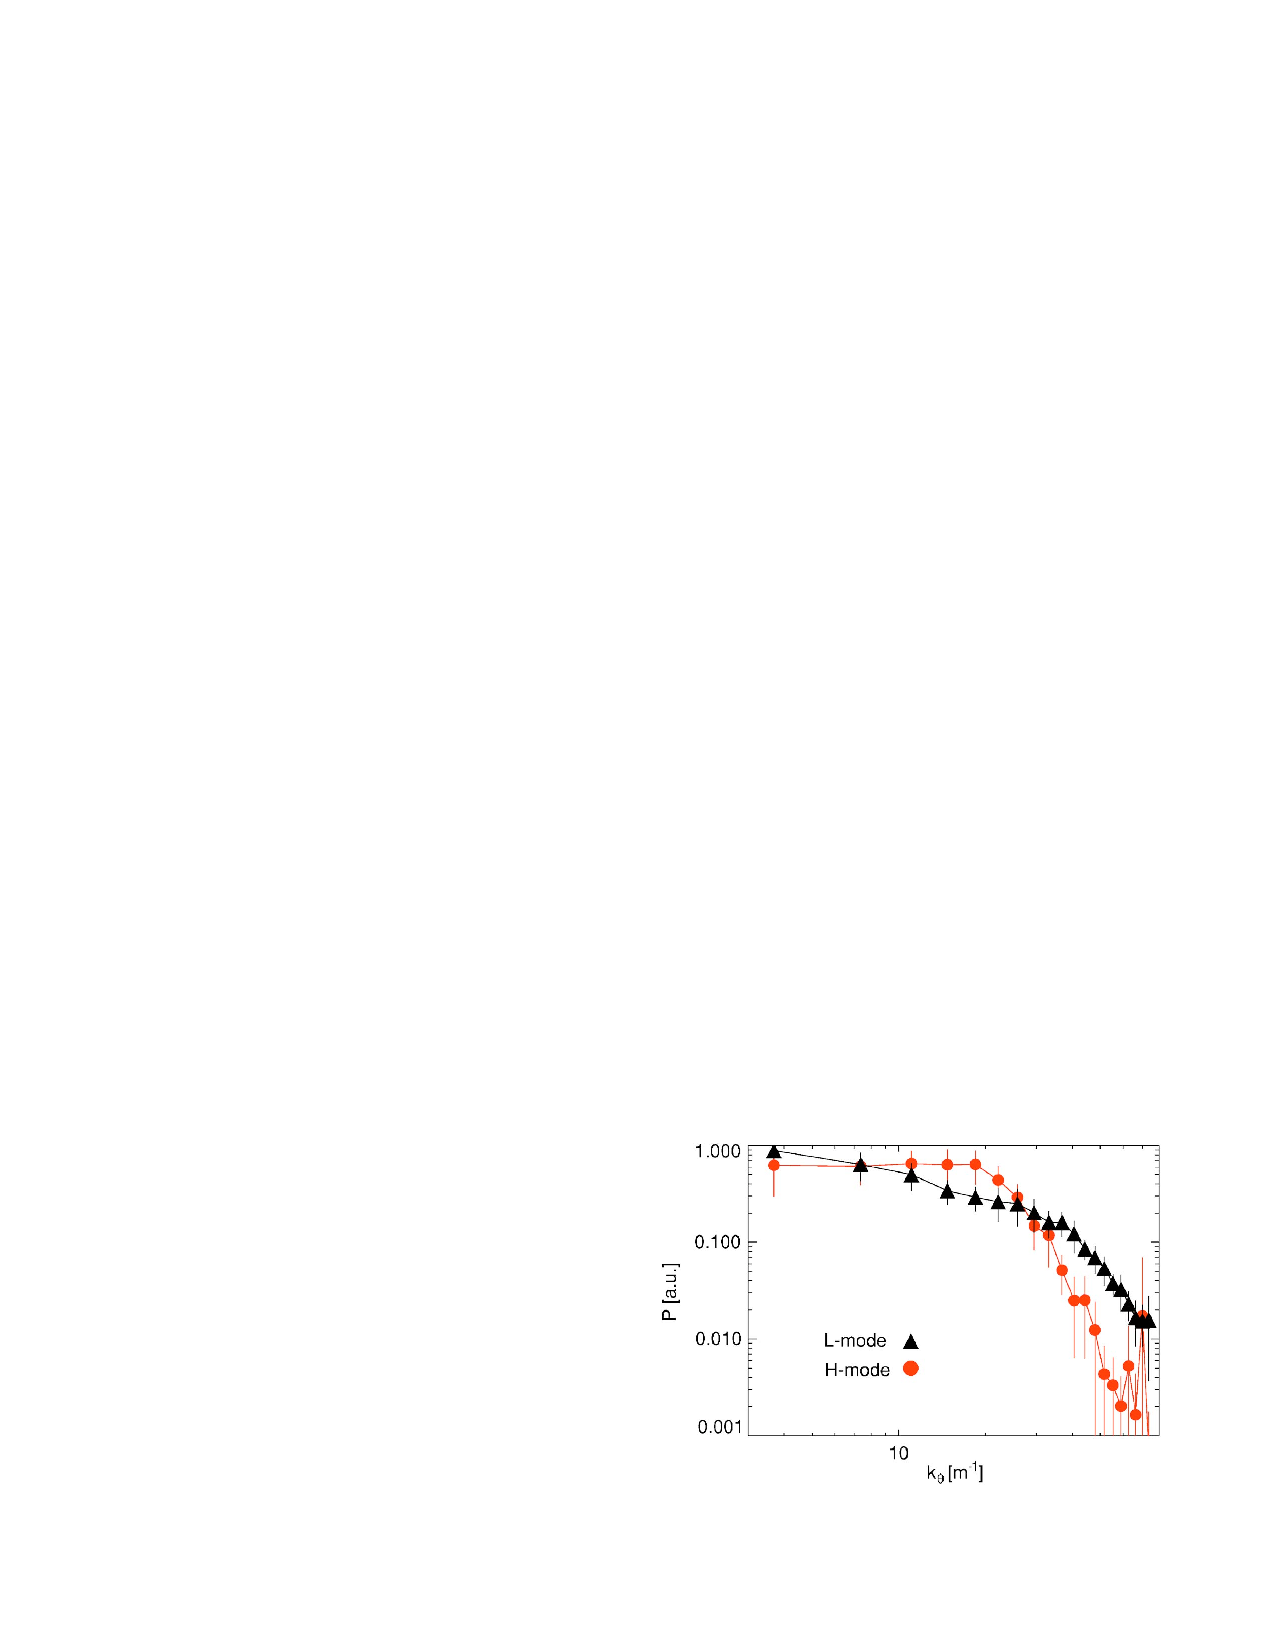
\includegraphics[height=4.5cm]{sk}}

\end{itemize}
}
\end{frame}

\begin{frame}{Beyond Fourier: Wavelet transform}
%% per aggiungere la lettera colorata con l'argomento in alto a sx'
\begin{tikzpicture}[remember picture, overlay]
\node [shift={(-0.779 cm,-0.3cm)}]  at (current page.north east)
   {\tikz[baseline=(t1.base)]{\node[fill=tascarletred](t1){%
{\large D}};}
    };
\end{tikzpicture}
%%
%\setbeamercovered{transparent=10}
\begin{itemize}[<+->]
\item {\small  The Fourier decomposition uses trigonometric functions as
  orthogonal basis}
\item {\small  These functions oscillates forever,
  i.e. the information spreaded} 
\item {\small  We need functions localized in time and scales $\Rightarrow$
  \textcolor{tachameleon}{\texttt{Wavelet
      Transform}} {\footnotesize \parencite{Farge:1992un,Mallat:1999te}}.
}
\begin{center}
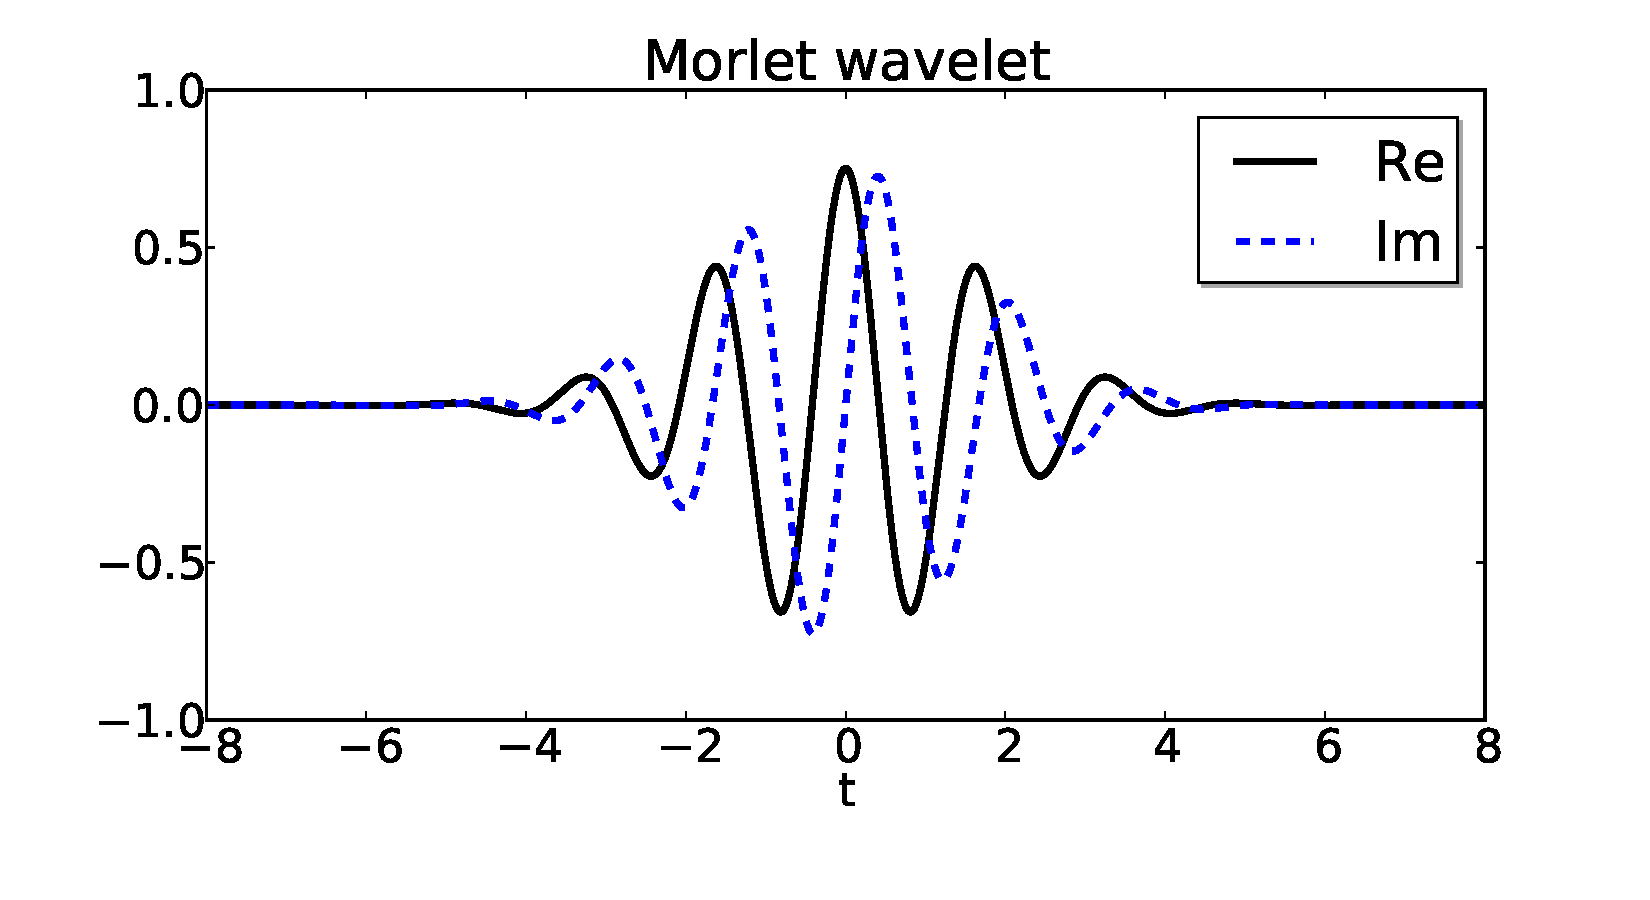
\includegraphics[height=3.5cm]{morlet}
\end{center}

\item {\small  Defining time-frequency atoms as
  $\psi_{s,\tau}=\frac{1}{\sqrt{\tau}}\psi\left(\frac{t-s}{\tau}\right)$ the
  \textcolor{tachameleon}{\texttt{Continuous Wavelet Transform}} is
  defined as }
\begin{equation*}
w(s,\tau)=\frac{1}{\sqrt{\tau}}\int_{-\infty}^{+\infty}f(t)\psi^{*}\left(\frac{t-s}{\tau}\right)dt
\end{equation*}
\end{itemize}
\end{frame}

\begin{frame}{Wavelet application}
%% per aggiungere la lettera colorata con l'argomento in alto a sx'
\begin{tikzpicture}[remember picture, overlay]
\node [shift={(-0.779 cm,-0.3cm)}]  at (current page.north east)
   {\tikz[baseline=(t1.base)]{\node[fill=tascarletred](t1){%
{\large D}};}
    };
\end{tikzpicture}
%%

\begin{itemize}
\item In analogy to Fourier we can define Wavelet Cross power spectrum
  and Corresponding phase spectrum (well localized in time/frequency)

\begin{center}
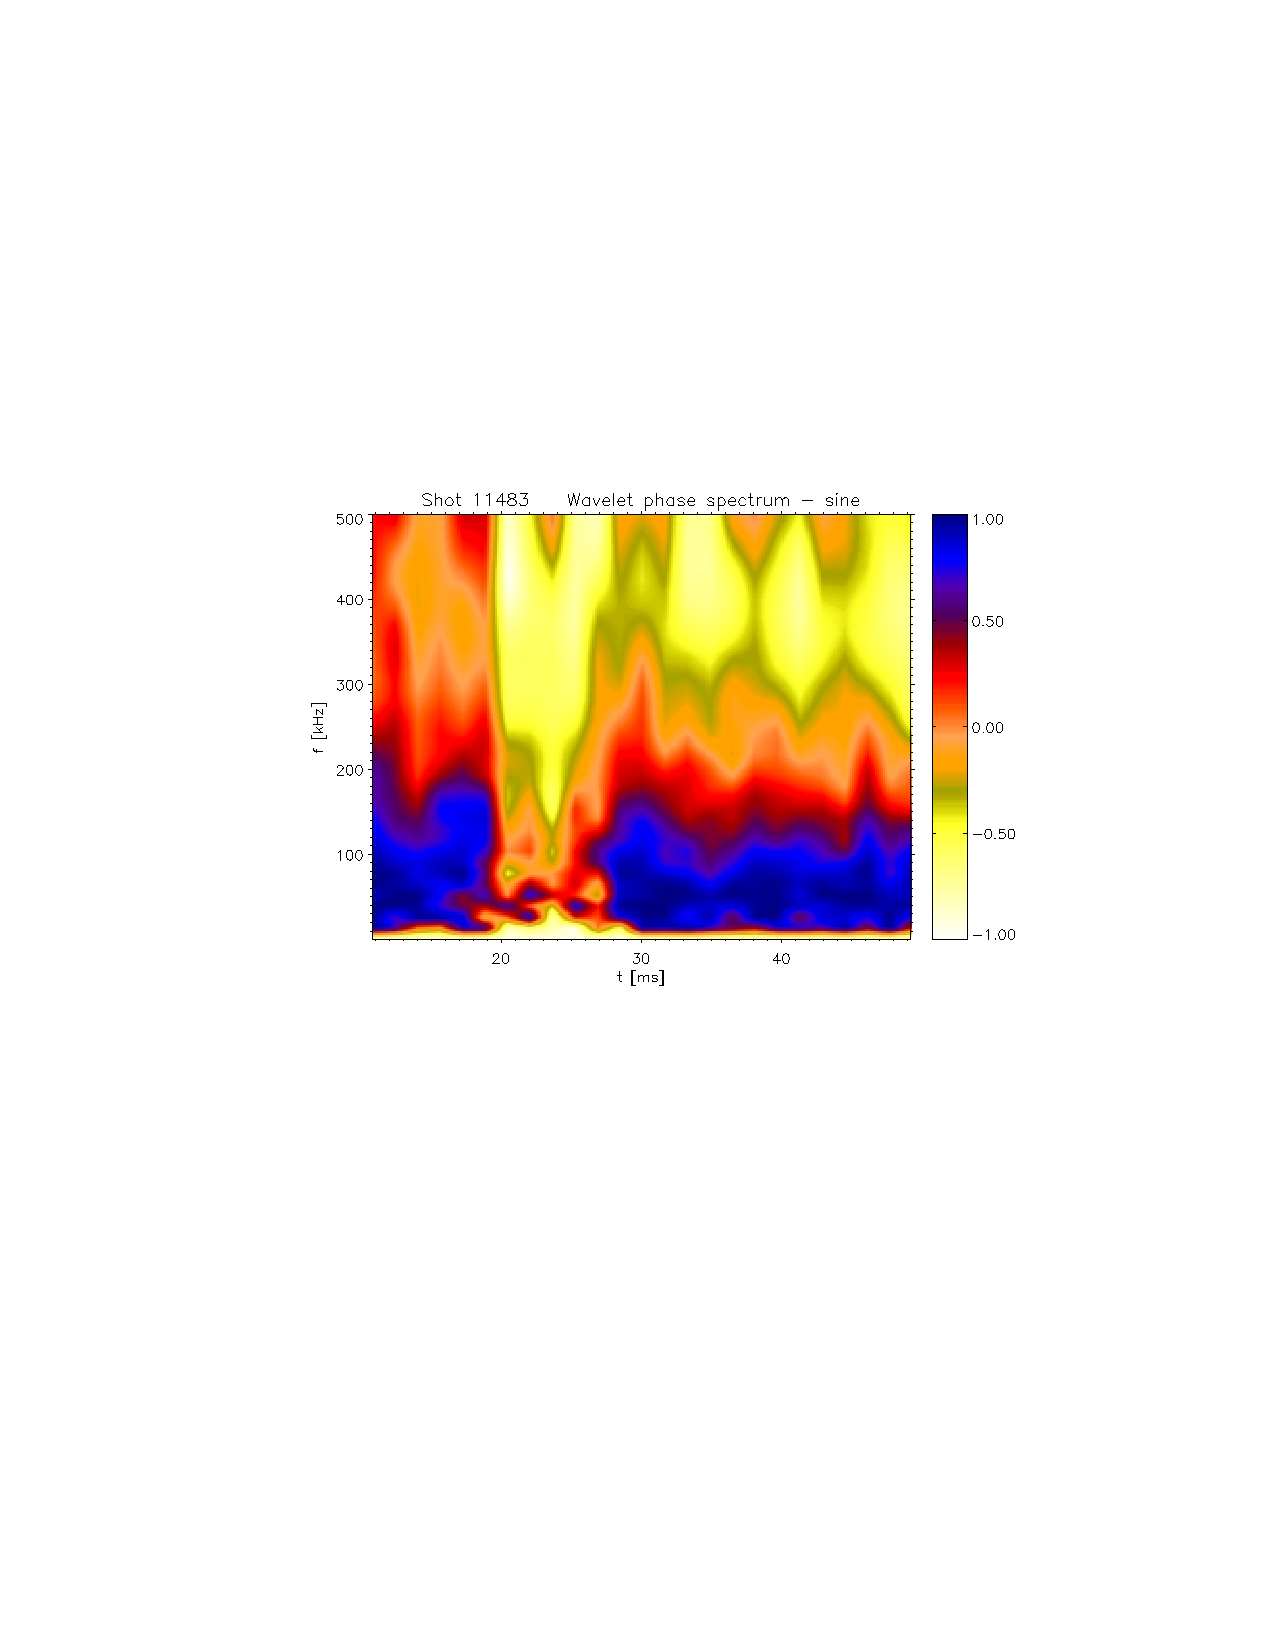
\includegraphics[height=3.5cm]{wavelet-phase}
\end{center}

\item Phase spectrum between density and potential varies because of
  variation of the shear $\rightarrow$ responsible for transport
  reduction {\footnotesize\parencite{Antoni:2000bn}}

\end{itemize}
\end{frame}


\begin{frame}{Wavelet for turbulence analysis}
%% per aggiungere la lettera colorata con l'argomento in alto a sx'
\begin{tikzpicture}[remember picture, overlay]
\node [shift={(-0.779 cm,-0.3cm)}]  at (current page.north east)
   {\tikz[baseline=(t1.base)]{\node[fill=tascarletred](t1){%
{\large D}};}
    };
\end{tikzpicture}
%%

%\setbeamercovered{transparent=10} 
 \begin{itemize}[<+->]
  \item Wavelet coefficients exhibit similar
    scaling properties as the fluctuations of the signals at the same
\begin{equation*}
\delta_{\tau} f = f(t+\tau)-f(t) \sim \tau^h \Rightarrow |w(t,\tau)|\sim\tau^{h+1/2}
\end{equation*}
% \item Thus wavelet coefficients may be used for the study of the
%   scaling properties of the fluctuation
\item Easy way to compute the
  \textcolor{tachameleon}{\texttt{Probability Distribution Function}}
  of normalized flutuations $C(t,\tau)=\frac{w(t,\tau)-\langle
    w(t,\tau)\rangle}{\sigma_{\tau}}$. For
  \textcolor{taskyblue}{self-similar} fluctuations, these should
  collapse to a single form

\item \textcolor{tascarletred}{\textbf{Revealing non
      self-similariy i.e. Intermittency}}

\begin{center}
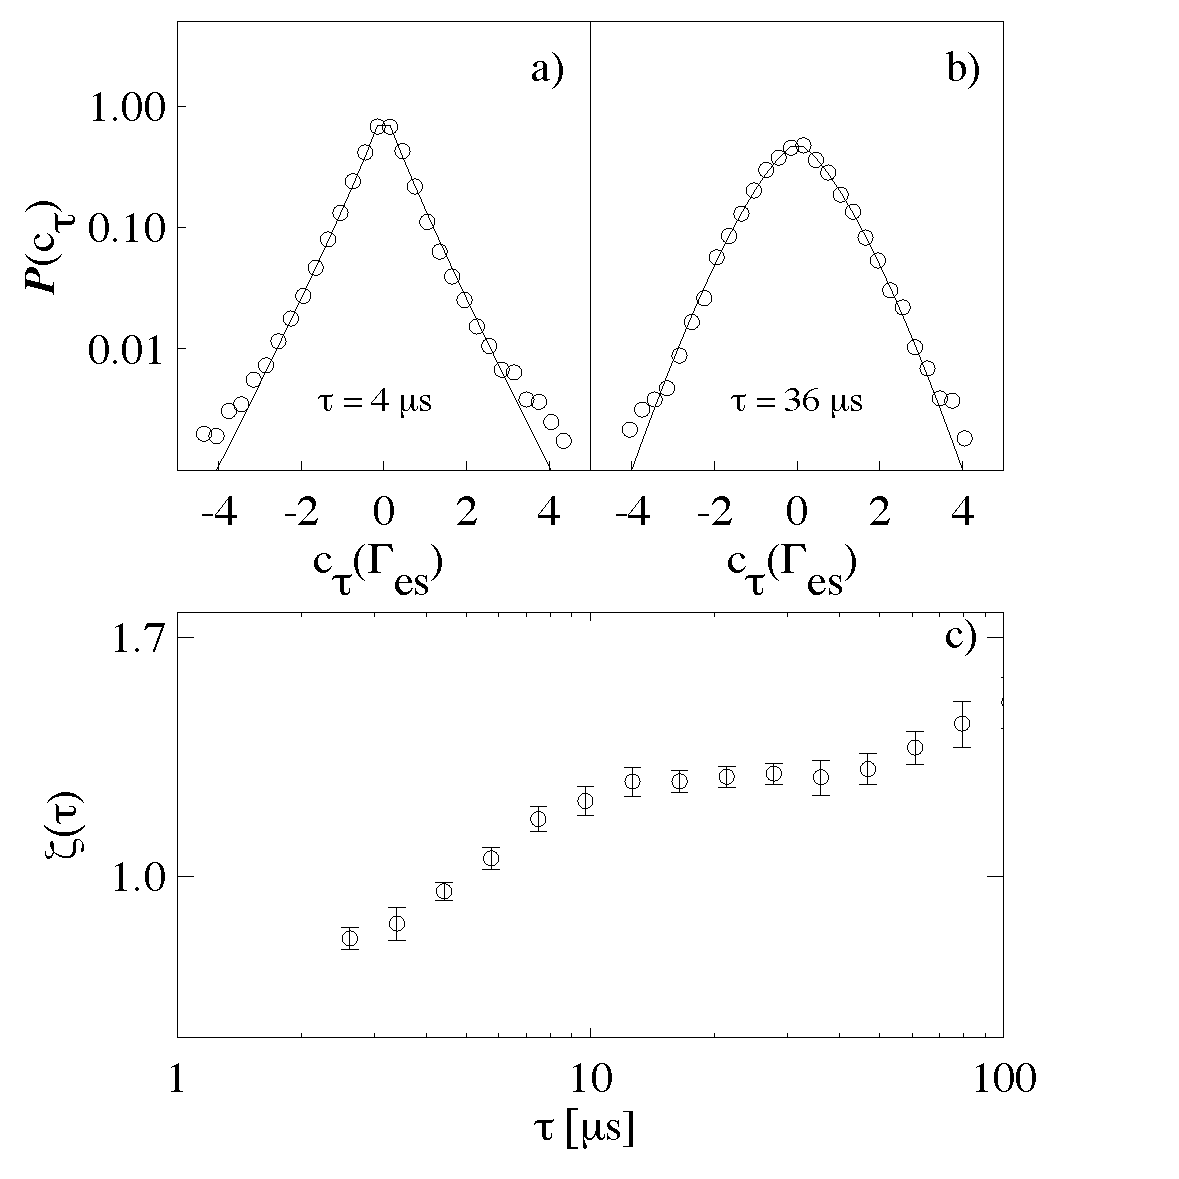
\includegraphics[height=3.7cm]{pdf_fluct}
\end{center}

\end{itemize}
\end{frame}

% \begin{frame}
 %  \frametitle{Local Intermittency Measurements}
% %% per aggiungere la lettera colorata con l'argomento in alto a sx'
% \begin{tikzpicture}[remember picture, overlay]
% \node [shift={(-0.779 cm,-0.3cm)}]  at (current page.north east)
%    {\tikz[baseline=(t1.base)]{\node[fill=tascarletred](t1){%
% {\large D}};}
%     };
% \end{tikzpicture}
% %%

%   \begin{itemize}
% \item Intermittency is due to the presence of strong, sporadic fluctuations
% \item The \textcolor{ta3chameleon}{\texttt{Local Intermittency
%       Measurements}} is a threshold method, based on wavelet, which identifies \alert{in time and
%   scales} these fluctuations {\footnotesize\parencite{Antoni:2001tm}}

% \item The typical shape of the fluctuations may be derived using
%   \textcolor{ta3chameleon}{\texttt{Conditional Average Procedure}},
%   i.e. averaging different time windows of the signal 
% \only<2>{\item Shape of a typical  \alert{Intermittent Events} or
%   \alert{blobs}
% \begin{center}
% 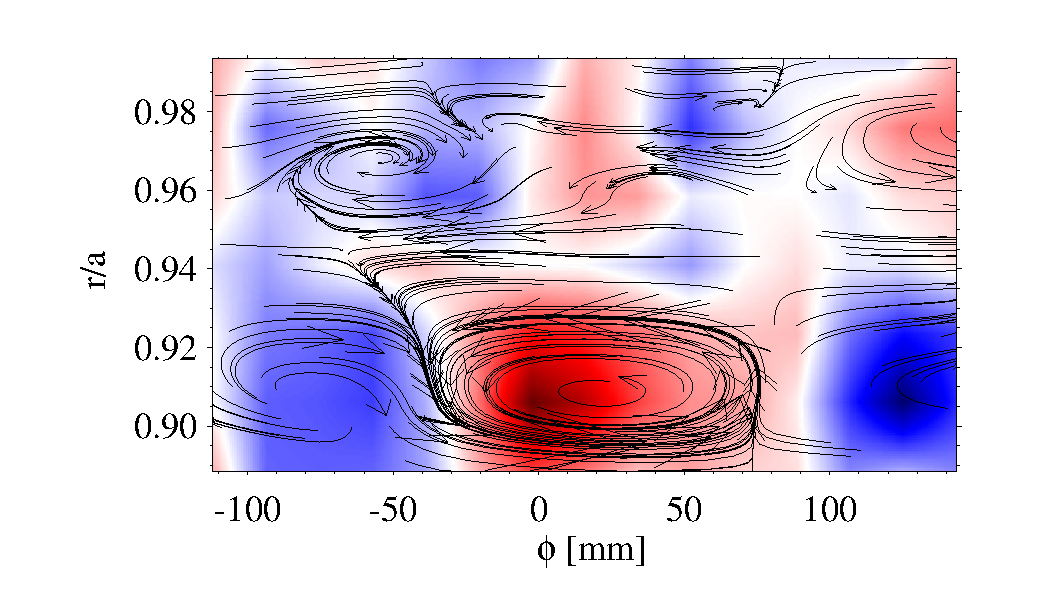
\includegraphics[height=3.6cm]{campo_vortici}
% \end{center}}
% \end{itemize}
% \end{frame}


\begin{frame}{Summary}
\begin{itemize}
{\large\item High temporal and spatial resolution are needed for better
  characterization of the plasma. But two points still gives a bunch
  of information
\item Fourier transform allows estimate of quantities directly
  comparable with theories
\item Often localized events (in space or time) require more
  sophisticated tools which maintain the locality of the information
\item As much as possible correlation between different diagnostics
  are generally needed for an appropriate comprehension}
\end{itemize}

\end{frame}
\begin{frame}[allowframebreaks]{Bibliography}
\printbibliography
\end{frame}

\end{document}
